% ============================================================
% 融合特征匹配与异常行为分析的网络攻击检测系统 — 总体设计报告
% 编译方式: xelatex paper.tex
% ============================================================

\documentclass[12pt,a4paper]{ctexart}

% ---- 页面设置 ----
\usepackage[top=2.5cm, bottom=2.5cm, left=2.8cm, right=2.8cm]{geometry}
\usepackage{setspace}
\onehalfspacing

% ---- 基础宏包 ----
\usepackage{graphicx}
\usepackage{booktabs}
\usepackage{multirow}
\usepackage{hyperref}
\usepackage{xcolor}
\usepackage{enumitem}
\usepackage{caption}
\usepackage{float}
\usepackage{listings}
\usepackage{fancyhdr}
\usepackage{lastpage}

% ---- 超链接 ----
\hypersetup{
    colorlinks=true,
    linkcolor=black,
    citecolor=blue,
    urlcolor=blue,
}

% ---- 代码块样式 ----
\lstset{
    basicstyle=\ttfamily\footnotesize,
    breaklines=true,
    frame=single,
    numbers=none,
    showstringspaces=false,
    tabsize=2,
    captionpos=b,
    language=,
}
% 定义 json 和 bash 语言（listings 基础包不含它们）
\lstdefinelanguage{json}{
    morestring=[b]",
    morestring=[d]{'},
}
\lstdefinelanguage{bash}{
    morekeywords={python, if, else, fi, for, while, do, done},
    alsoletter={-},
}

% ---- 修复 fancyhdr headheight 警告 ----
\setlength{\headheight}{15pt}

\begin{document}

% ---- 封面 ----
\begin{titlepage}
\thispagestyle{empty}

\vspace*{3cm}

\begin{center}
{\Huge \textbf{融合特征匹配与异常行为分析的}} \\[0.6em]
{\Huge \textbf{网络攻击检测系统}} \\[1.2em]
{\LARGE —— 总体设计报告 ——}
\end{center}

\vspace{3cm}

\begin{center}
\renewcommand{\arraystretch}{1.2}
\begin{tabular}{rl}
    \textbf{项目名称} & 融合特征匹配与异常行为分析的网络攻击检测系统 \\[0.3em]
    \textbf{组\hspace{2em}长} & 韩宇飞 \quad 524031910172 \\[0.3em]
    \textbf{成\hspace{2em}员} & 李哲 \quad 524031910017 \\[0.3em]
                             & 曾子恒 \quad 523010910022 \\[0.3em]
                             & 陈志恒 \quad 524031910111 \\[0.3em]
                             & 姜新晨 \quad 524031910769 \\[0.5em]
    \textbf{学\hspace{2em}院} & 计算机学院 \\[0.3em]
    \textbf{指导教师} & 陈秀真 \quad 姚立红 \\[0.5em]
    \textbf{日\hspace{2em}期} & 2026年7月17日 \\
\end{tabular}
\end{center}

\vfill
\begin{center}
{\small \textcolor{gray}{上海交通大学 · 计算机学院 · 信息安全科技创新课程}}
\end{center}
\end{titlepage}

% ---- 全局页眉页脚设置 ----
\pagestyle{fancy}
\fancyhf{}
\fancyhead[L]{\small 融合特征匹配与异常行为分析的网络攻击检测系统}
\fancyhead[R]{\small 总体设计报告}
\renewcommand{\headrulewidth}{0.4pt}
\fancyfoot[C]{\small —\ \thepage\ —}
\renewcommand{\footrulewidth}{0pt}

% 封面和目录页用 plain 风格（无页眉线）
\fancypagestyle{plain}{
    \fancyhf{}
    \fancyfoot[C]{\small —\ \thepage\ —}
    \renewcommand{\headrulewidth}{0pt}
}

% ---- 目录 ----
\newpage
\pagenumbering{Roman}  % 目录用罗马数字
\tableofcontents
\newpage

\pagenumbering{arabic}  % 正文用阿拉伯数字
\setcounter{page}{1}

% ============================================================
% 一、系统需求分析
% ============================================================
\section{系统需求分析}

\subsection{安全需求}

本系统面向小型网络环境（如实验室局域网、校内子网段），需解决以下四类安全检测问题：

\subsubsection{已知 Web 攻击识别}

网络中存在大量具有固定特征的攻击行为，如 SQL 注入（\texttt{UNION SELECT}、\texttt{' OR 1=1}）、跨站脚本 XSS（\texttt{<script>} 标签注入）、恶意系统命令执行（\texttt{/bin/cat /etc/passwd}）等。这些攻击以 HTTP 请求为载体，传统包过滤防火墙工作在网络层/传输层，无法检测应用层载荷中的恶意特征。系统需内置一个可维护、可扩展的攻击特征库，对实时流量的应用层 payload 进行多模式匹配，且支持字面匹配（literal）和正则表达式匹配（regex）两种模式。

\subsubsection{暴力破解行为发现}

面向 SSH（22端口）、FTP（21端口）、数据库（3306、5432、6379端口）、Web 登录（8080、8443端口）等认证服务的暴力密码枚举攻击极为常见。攻击者在短时间内以极高频率发起连接尝试，表现为同一源 IP 在几十秒内对同一目标登录端口发起数十次 TCP SYN。系统需基于时间窗口的滑动密度统计自动发现此类行为，并结合服务端 RST 拒绝响应的次数佐证认证失败。

\subsubsection{网络扫描与横向扩散识别}

攻击者在渗透阶段通常在信息搜集后进行端口扫描（发现开放服务）和内网横向移动（跳板攻击）。端口扫描表现为单一源 IP 在短时间内访问大量不同目标端口（24端口以上/60秒），横向扩散表现为单台内网主机在数分钟内访问多个不同内网 IP。系统需建立正常流量行为基线，识别上述显著偏离的探测行为。

\subsubsection{异常外联与 C2 通信检测}

受控主机（僵尸节点）可能向外部 C2 服务器发起隐蔽通信。这类连接在正常业务流量中不常见——内网主机通常不主动访问陌生公网 IP。系统需维护内网 IP 段白名单，识别内网主机向不在白名单中的公网 IP 发起的出站连接。

\subsection{具体功能要求}

系统按功能分解为五个模块，对应五位成员分工开发：

\begin{table}[H]
\centering
\caption{系统功能模块划分}
\label{tab:modules}
\small
\begin{tabular}{@{}cllp{5.5cm}@{}}
\toprule
编号 & 模块名称 & 负责人 & 核心功能 \\
\midrule
M1 & 数据包捕获与协议解析 & 李哲 & 实时/离线抓包、协议字段解析、TCP流重组、payload提取、TLS基础识别 \\
M2 & 特征行为检测引擎     & 曾子恒 & 特征库加载、字面/正则双模式匹配、同源同类60s窗口聚合为行为告警 \\
M3 & 暴力破解检测模块     & 陈志恒 & SYN连接收集+退化flow\_id计数、双指针滑动窗口密度统计、RST拒绝佐证 \\
M4 & 异常行为检测模块     & 姜新晨 & 端口扫描检测（同源端口多样性）、异常外联检测（内网IP白名单匹配） \\
M5 & 告警汇总与监控GUI    & 韩宇飞 & 多源告警合并/排序/去重、攻击行为关联、三页签GUI面板 \\
\bottomrule
\end{tabular}
\end{table}

各模块通过统一的 JSON 接口（报文记录格式 + 告警记录格式）松耦合通信。Phase1--3阶段所有检测模块的输入统一来自 \texttt{mock\_data/mock\_packets.json}（108条覆盖7类场景的模拟报文），Phase4起替换为真实抓包输出。

\subsection{开发平台要求}

\begin{table}[H]
\centering
\caption{开发平台选型}
\small
\begin{tabular}{@{}llp{6.5cm}@{}}
\toprule
项目 & 选型 & 选型理由 \\
\midrule
开发语言   & Python $\ge$ 3.9        & 生态丰富，scapy/pytest/tkinter 均为主流库 \\
抓包库     & scapy $\ge$ 2.5.0       & Python 原生，支持实时抓包与 pcap 离线解析 \\
GUI框架    & tkinter（标准库）        & 零依赖，ttk 主题化组件 \\
测试框架   & pytest $\ge$ 7.0        & 简洁断言，fixture 复用 mock 数据 \\
版本控制   & Git + GitHub Flow       & Feature 分支开发，PR 合并 \\
代码格式化 & black + isort           & 推荐，统一代码风格 \\
AI辅助     & Claude Code / Cursor / Trae / 通义灵码 & 提升开发效率，尤其在算法实现和测试生成方面 \\
\bottomrule
\end{tabular}
\end{table}

\subsection{运行环境要求}

\textbf{软件环境}：
\begin{itemize}[nosep]
    \item 操作系统：Linux（推荐 Ubuntu 22.04 LTS）或 Windows 10/11 + WSL2
    \item Python 3.9 及以上版本
    \item pip 依赖：\texttt{scapy>=2.5.0}, \texttt{pytest>=7.0.0}
    \item 实时抓包场景需安装 Npcap（Windows）或 libpcap（Linux）
\end{itemize}

\textbf{硬件环境}：
\begin{itemize}[nosep]
    \item 普通 PC 或笔记本，CPU 双核及以上，内存 $\ge$ 4GB
    \item 网卡支持混杂模式（Promiscuous Mode），用于实时抓包
    \item 若在虚拟机中运行，需将网络适配器配置为桥接模式
\end{itemize}

\textbf{权限要求}：
\begin{itemize}[nosep]
    \item 实时抓包需 root 权限（Linux）或管理员权限（Windows）
    \item 仅读取 pcap 文件则无需提权
\end{itemize}

% ============================================================
% 二、计划进度安排
% ============================================================
\section{计划进度安排}

项目自 2026年7月8日启动，至 8月5日最终提交，共四周。

\begin{table}[H]
\centering
\caption{项目进度表}
\label{tab:schedule}
\begin{tabular}{@{}lll@{}}
\toprule
日期 & 里程碑 & 状态 \\
\midrule
7/9(四)--7/12(日) & 李哲交付 mock 数据(108条) + capture 模块 & $\checkmark$ 已完成 \\
7/13(一)--7/18(六) & 四人完成核心检测逻辑 & $\circlearrowright$ 进行中 \\
7/20(一)          & 接口对齐检查（aggregator 校验各模块告警格式） & $\square$ 待进行 \\
7/21(二)--7/22(三) & 单元测试编写 + 异常处理补充 & $\square$ 待进行 \\
7/23(四)--7/25(六) & 全链路联调（真实抓包替换mock）+ PR 合入 main & $\square$ 待进行 \\
7/26(日)--7/28(二) & PPT 制作 + 演示数据准备 + 内部预演 & $\square$ 待进行 \\
\textbf{7/29(三)}   & 课堂项目分享汇报 & $\square$ 待进行 \\
7/30(四)--8/1(六)  & 结题报告撰写 + 源码整理 & $\square$ 待进行 \\
\textbf{8/2(日)}    & 提前提交（比 8/5 截止早3天） & $\square$ 待进行 \\
8/3(一)--8/4(二)   & 缓冲时间，应对突发问题 & $\square$ 待进行 \\
\textbf{8/5(三)}    & 官方结题截止 & $\square$ 待进行 \\
\bottomrule
\end{tabular}
\end{table}

截至7月17日，李哲（capture）、陈志恒（bruteforce）、韩宇飞（aggregator+GUI）三个模块已完成并合入 main 分支。曾子恒（signature）和姜新晨（anomaly）两个检测模块正在开发中。

\begin{figure}[H]
\centering
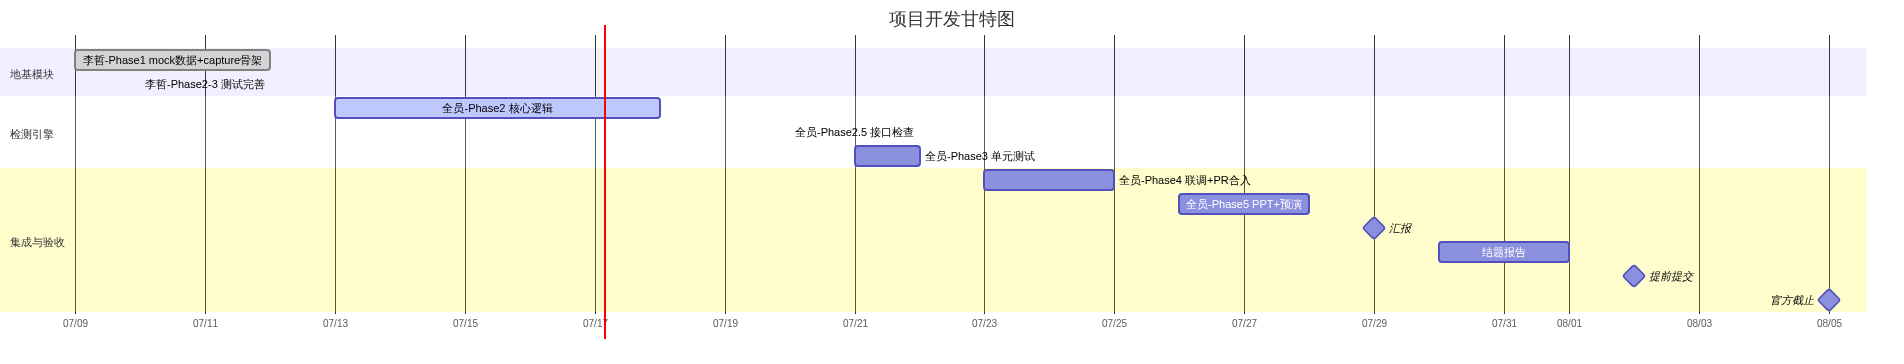
\includegraphics[width=\textwidth]{figures/01_gantt_schedule.png}
\caption{项目开发甘特图}
\label{fig:gantt}
\end{figure}

% ============================================================
% 三、系统总体架构
% ============================================================
\section{系统总体架构}

\subsection{平台架构}

系统采用自底向上的四层分层架构：数据捕获层 $\to$ 检测引擎层 $\to$ 汇总关联层 $\to$ 展示层。各层之间通过统一的 JSON 数据格式解耦。

\begin{table}[H]
\centering
\caption{四层架构各层职责}
\small
\begin{tabular}{@{}clp{8cm}@{}}
\toprule
层级 & 名称 & 职责与产出 \\
\midrule
L1 & 数据捕获层  & 从网卡/pcap获取报文，解析为标准化记录，完成TCP流重组。\textbf{产出：} Packet Record\texttt{[]} \\
L2 & 检测引擎层  & 三个引擎并行消费报文，从不同维度检测攻击行为。\textbf{产出：} Alert Record\texttt{[]} \\
L3 & 汇总关联层  & 合并多源告警，行为关联，赋予统一behavior\_id。\textbf{产出：} \texttt{merged\_alerts.json} \\
L4 & 展示层      & 以攻击行为为粒度展示，筛选/搜索/统计/特征库管理。\textbf{产出：} GUI窗口 \\
\bottomrule
\end{tabular}
\end{table}

\begin{figure}[H]
\centering
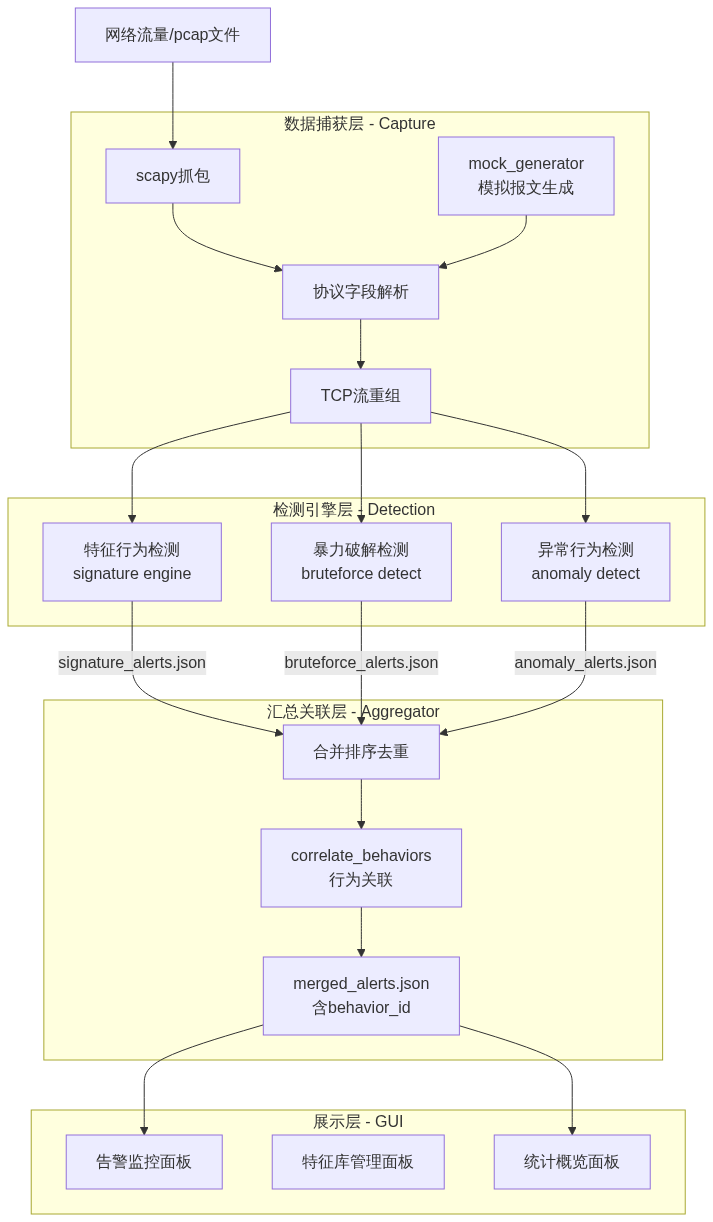
\includegraphics[width=\textwidth]{figures/02_platform_architecture.png}
\caption{系统四层平台架构}
\label{fig:platform}
\end{figure}

\subsection{功能架构与数据流}

系统核心数据流为：

\textbf{数据包捕获 $\to$ TCP重组/协议识别 $\to$ 并行检测（特征行为检测 $\parallel$ 暴力破解检测 $\parallel$ 异常行为检测）$\to$ 行为告警关联与汇总 $\to$ 监控GUI。}

\begin{figure}[H]
\centering
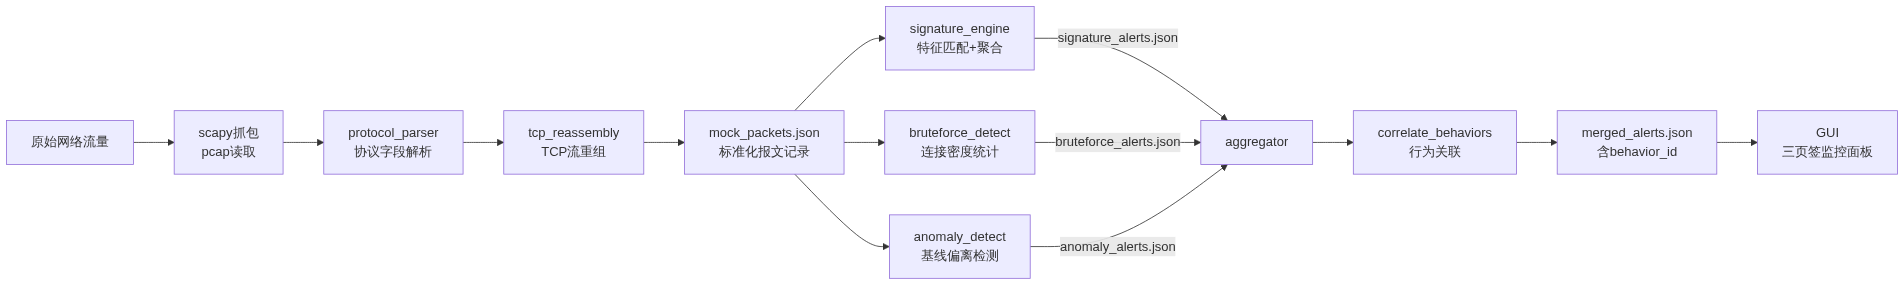
\includegraphics[width=\textwidth]{figures/03_dataflow_overview.png}
\caption{系统数据流全景图}
\label{fig:dataflow}
\end{figure}

\textbf{关键设计决策}：

\begin{enumerate}[nosep]
    \item \textbf{并行检测架构}：三个检测引擎独立运行，彼此不依赖对方的输出。这允许任一引擎单独测试和部署，也允许未来增加新的检测引擎而不影响现有模块。
    \item \textbf{统一的 JSON 接口}：所有模块通过两个标准 JSON Schema（Packet Record 和 Alert Record）通信。模块间不直接导入彼此的 Python 代码，仅通过 JSON 文件交换数据。这保证了即使独立开发者使用不同的代码风格或第三方库，也不会产生依赖冲突。
    \item \textbf{行为聚合而非逐包告警}：无论是特征匹配、暴力破解还是异常检测，最终产出都以"攻击行为事件"为粒度。特征引擎对同源同类命中做窗口聚合，暴力破解按（src\_ip, dst\_ip, dst\_port）分组，异常检测以偏离行为为单位。这使得 GUI 展示的告警数量可控、可读，避免告警洪流。
    \item \textbf{CLI + 全链路两种运行模式}：每个检测模块提供独立的 \texttt{python -m} CLI入口（\texttt{--input} / \texttt{--output}），便于单模块调试；同时 \texttt{main.py} 提供一键运行全链路的入口，用于集成测试和演示。
\end{enumerate}

% ============================================================
% 四、模块一：数据捕获与协议解析
% ============================================================
\section{系统功能模块一：数据捕获与协议解析（李哲）}

\subsection{模块结构与调用关系}

\begin{verbatim}
src/capture/
├── __init__.py
├── packet_capture.py      # 抓包入口：capture_live() / read_pcap()
├── protocol_parser.py     # 协议解析核心
├── tcp_reassembly.py      # TCP流重组
└── mock_generator.py      # Mock数据生成器
\end{verbatim}

子模块调用关系：\texttt{packet\_capture} $\to$ \texttt{protocol\_parser.parse\_packet()} $\to$ \texttt{tcp\_reassembly.reassemble()} $\to$ 标准化记录列表。

\begin{figure}[H]
\centering
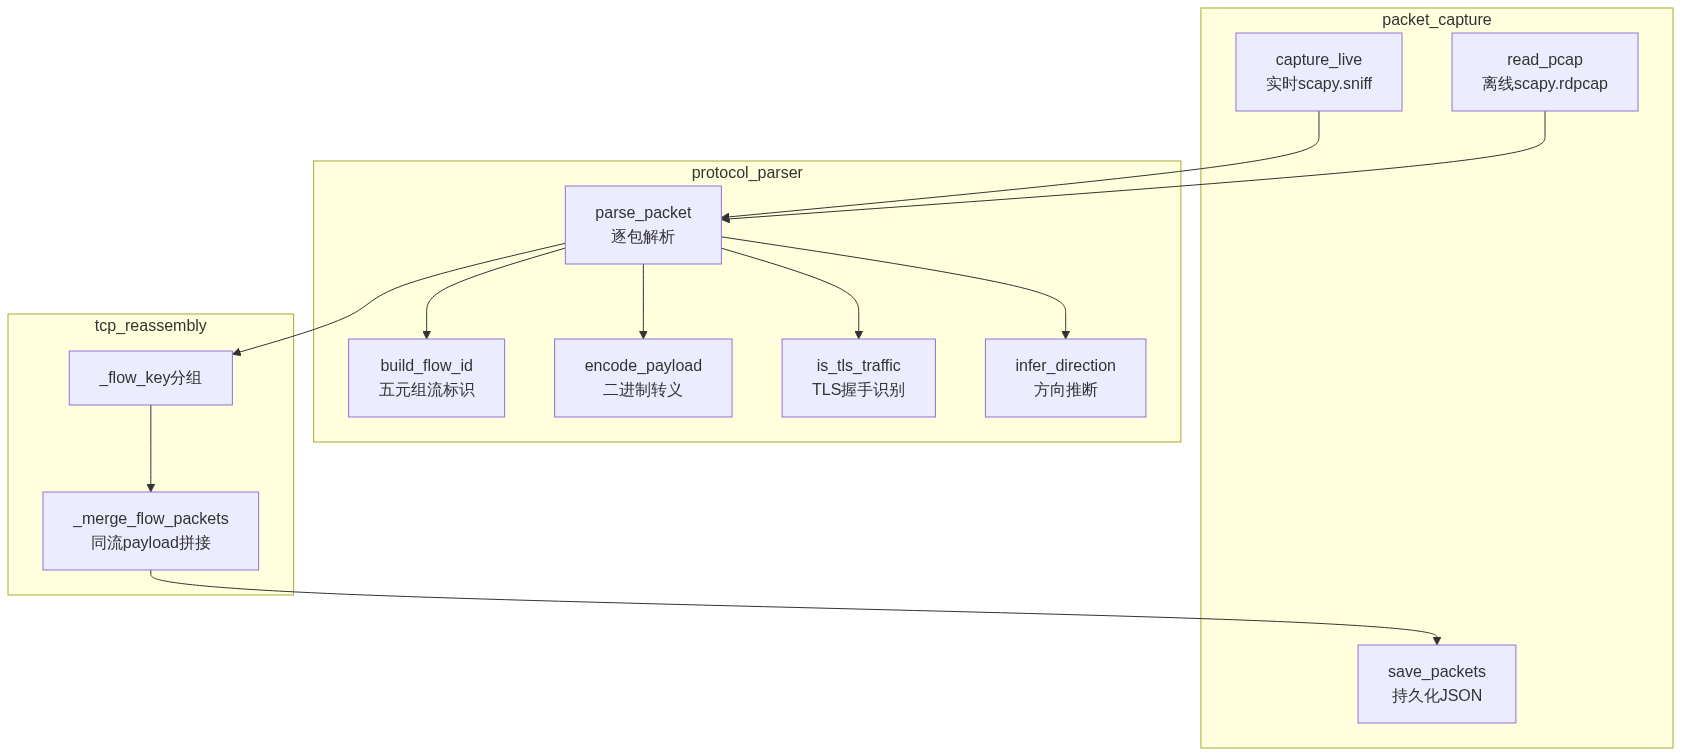
\includegraphics[width=\textwidth]{figures/04_capture_internal.png}
\caption{capture 模块内部调用关系}
\label{fig:capture}
\end{figure}

\subsection{报文捕获子模块（packet\_capture.py）}

\textbf{实时抓包} \texttt{capture\_live(interface, count, timeout, do\_reassemble)}：
\begin{itemize}[nosep]
    \item 底层调用 \texttt{scapy.all.sniff(iface=interface, count=count, timeout=timeout)} 从指定网卡捕获原始报文
    \item \texttt{count=0} 时表示不限数量，由 \texttt{timeout} 参数控制抓包时长
    \item 捕获完成后逐包调用 \texttt{parse\_packet()} 解析，可选调用 \texttt{reassemble()} 进行TCP重组
    \item scapy 未安装时打印 ERROR 日志并返回空列表，不崩溃
\end{itemize}

\textbf{离线读取} \texttt{read\_pcap(filepath, do\_reassemble)}：
\begin{itemize}[nosep]
    \item 调用 \texttt{scapy.all.rdpcap(filepath)} 读取 pcap/pcapng 文件
    \item 文件不存在时打印 WARNING 日志并返回空列表
\end{itemize}

\textbf{CLI入口}：
\begin{lstlisting}
# 离线模式
python -m src.capture.packet_capture \
    --pcap capture.pcap --output results/captured_packets.json
# 实时模式
python -m src.capture.packet_capture \
    --live --interface eth0 --count 100 --timeout 30
# 跳过TCP重组
python -m src.capture.packet_capture --pcap capture.pcap --no-reassemble
\end{lstlisting}

\subsection{协议解析与流重组子模块}

\begin{figure}[H]
\centering
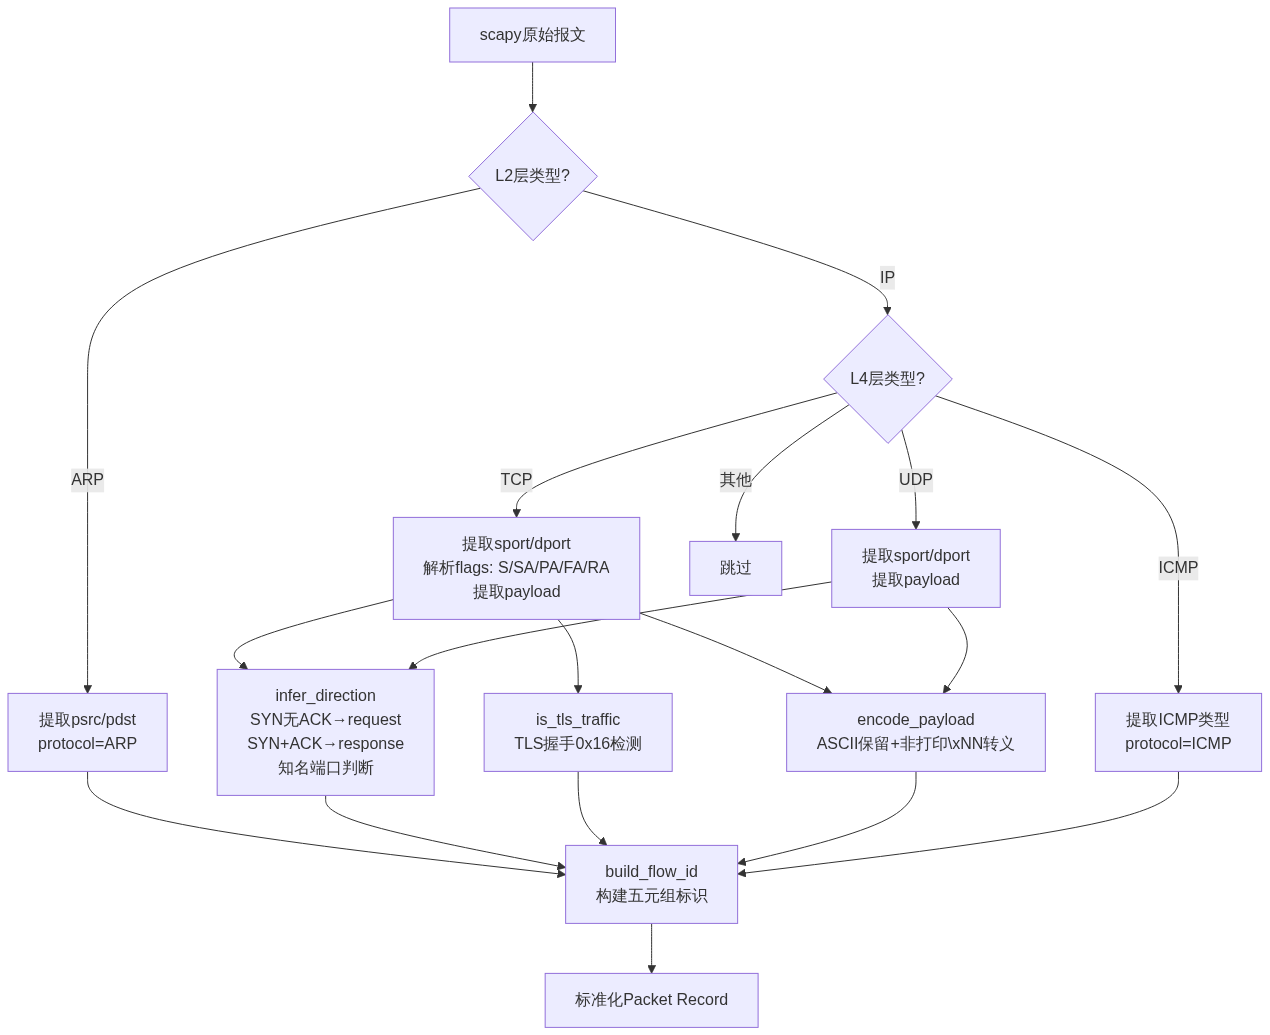
\includegraphics[width=\textwidth]{figures/05_parse_packet.png}
\caption{parse\_packet 协议栈解析流程}
\label{fig:parse}
\end{figure}

\textbf{关键字段解析规则}：

\begin{itemize}[nosep]
    \item \texttt{timestamp}：从 scapy 报文的 \texttt{.time} 属性提取，格式化为 ISO8601 毫秒精度
    \item \texttt{flow\_id}：\texttt{\{src\_ip\}:\{src\_port\}->\{dst\_ip\}:\{dst\_port\}/\{protocol\}}
    \item \texttt{direction}：优先通过 TCP flags 判断（SYN无ACK $\to$ request，SYN+ACK $\to$ response），其次通过知名服务端口列表判断
    \item \texttt{flags}：将 scapy 的 TCP flag 位映射为紧凑字符串（F/S/R/P/A/U/E/C）
    \item \texttt{payload}：可打印 ASCII(32--126)和空格/TAB/回车/换行直接保留，其余字节转为 \texttt{\textbackslash xNN} 形式
    \item \texttt{payload\_len}：线路上原始 TCP/UDP 数据段的字节长度，非转义后字符串长度
\end{itemize}

\textbf{TLS流量识别（加分项）} \texttt{is\_tls\_traffic(payload, src\_port, dst\_port)}：
\begin{itemize}[nosep]
    \item 检测 TLS 记录层 ContentType=0x16（Handshake）且 Version $\in$ \{0x0300, 0x0301, 0x0302, 0x0303\}
    \item 辅助检测：当端口为 443/8443/465/993/995 时，增强置信度判断
    \item 识别到 TLS 流量时打印 DEBUG 日志标记
\end{itemize}

\textbf{TCP流重组} \texttt{reassemble(packets)}：
\begin{itemize}[nosep]
    \item 将报文按 \texttt{flow\_id} 分组为 TCP 流（非TCP报文原样保留）
    \item 每条流内按 timestamp 排序后，区分数据报文（\texttt{payload\_len>0}）和控制报文（SYN/FIN/RST 无数据）
    \item 数据报文合并：拼接所有 payload 字符串、累加 \texttt{payload\_len}，以流中首条报文的时间戳和地址信息为代表
    \item 控制报文原样输出不合并（保留连接建拆的时序信息供检测模块使用）
    \item 输出按 timestamp 重新排序
\end{itemize}

\subsection{Mock 数据生成器（mock\_generator.py）}

\texttt{generate\_mock\_packets()} 函数以 \texttt{datetime(2026,7,8,10,0,0)} 为基准时间，通过工厂函数 \texttt{\_pkt()} 逐条构造报文，时间戳以 50ms 步进，确保每条报文时间唯一且有序。

\begin{table}[H]
\centering
\caption{Mock 数据场景覆盖对照表}
\label{tab:mock}
\small
\begin{tabular}{@{}lp{2.8cm}p{2.5cm}p{4.5cm}@{}}
\toprule
场景 & 数量 & 关键特征 & 预期检出模块 \\
\midrule
正常HTTP流量 & 8条  & GET/POST请求+响应 & 均不应告警 \\
正常SSH流量 & 4条  & SSH banner+握手 & 均不应告警 \\
正常FTP流量 & 6条  & USER/PASS/LIST命令 & 均不应告警 \\
正常DNS+ICMP & 4条  & UDP DNS + ICMP echo & 均不应告警 \\
SQL注入特征 & 7条  & UNION SELECT, 'OR 1=1 & signature \\
XSS特征     & 6条  & <script>, <SCRIPT> & signature \\
木马/恶意命令 & 4条 & /bin/cat, /etc/passwd & signature \\
暴力破解SSH & 36条 & 18次SYN+18次RST & bruteforce \\
端口扫描    & 24条 & 24个不同端口SYN探测 & anomaly \\
异常外联    & 3条  & 内网IP连陌生公网IP & anomaly \\
正常HTTPS   & 1条  & TLS ClientHello & 均不应告警 \\
\bottomrule
\end{tabular}
\end{table}

\textbf{合计：108条}，覆盖全部7类需求场景。

% ============================================================
% 五、模块二：特征行为检测引擎
% ============================================================
\section{系统功能模块二：特征行为检测引擎（曾子恒）}

\subsection{模块结构}

\begin{verbatim}
src/signature_engine/
├── __init__.py
├── signature_db.py    # 特征库管理
└── matcher.py         # 匹配引擎 + CLI
\end{verbatim}

\begin{figure}[H]
\centering
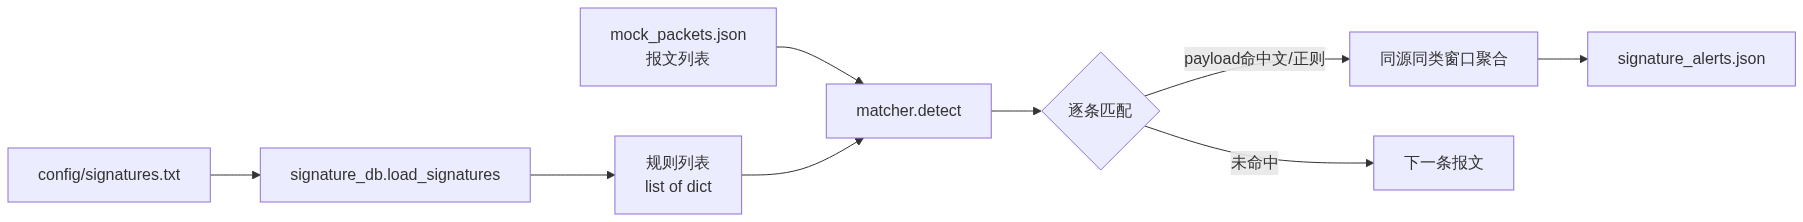
\includegraphics[width=\textwidth]{figures/06_signature_engine.png}
\caption{signature 模块结构与数据流}
\label{fig:sig-module}
\end{figure}

\subsection{特征库管理（signature\_db.py）}

\textbf{规则配置文件格式}（\texttt{config/signatures.txt}）：

\begin{lstlisting}
# 格式: 规则ID | 攻击类型 | 匹配模式 | 特征串 | 适用协议 | 严重程度
SIG-001 | SQL注入 | literal | UNION SELECT | HTTP | high
SIG-002 | SQL注入 | literal | ' OR 1=1 | HTTP | high
SIG-003 | XSS | regex | <script.*?>.*?</script> | HTTP | medium
SIG-004 | 恶意命令 | literal | /bin/cat%20/etc/passwd | HTTP | high
SIG-005 | 木马通信 | literal | /faxsurvey? | TCP | high
\end{lstlisting}

\textbf{加载逻辑} \texttt{load\_signatures(filepath)}：
\begin{itemize}[nosep]
    \item 按行读取，跳过空行和 \texttt{\#} 开头的注释行
    \item 以 \texttt{|} 分隔符拆分为6个字段
    \item 字段数不等于6的行打印 WARNING 跳过，不中断加载
    \item 返回值：\texttt{list[dict]}，每条规则包含上述6个键
\end{itemize}

\textbf{匹配模式说明}：
\begin{itemize}[nosep]
    \item \texttt{literal}：大小写不敏感的 \texttt{str.lower() in} 子串匹配，性能 O(n$\cdot$m)
    \item \texttt{regex}：使用 \texttt{re.search(pattern, payload, re.IGNORECASE)} 正则匹配
    \item 两者均可作为 baseline；高效多模式匹配（如 AC 自动机）是加分项
\end{itemize}

\subsection{匹配引擎（matcher.py）}

\textbf{行为聚合规则}：
\begin{itemize}[nosep]
    \item 分组键：\texttt{(src\_ip, category)}
    \item 窗口：默认60秒
    \item 同一分组内时间间隔 $\le$ 窗口的同类型告警共享一个 \texttt{behavior\_id}
    \item 作用：将逐包命中聚合为一个攻击行为事件，而非逐条报 N 个告警
\end{itemize}

\textbf{CLI入口}：
\begin{lstlisting}
python -m src.signature_engine.matcher \
    --input mock_data/mock_packets.json \
    --output results/signature_alerts.json
\end{lstlisting}

% ============================================================
% 六、模块三：暴力破解检测
% ============================================================
\section{系统功能模块三：暴力破解检测模块（陈志恒）}

\subsection{模块结构}

\begin{verbatim}
src/bruteforce_detect/
├── __init__.py
└── login_monitor.py    # 完整检测逻辑（单文件内聚）
\end{verbatim}

单文件内聚设计：所有辅助函数和检测逻辑集中在一个模块中，外部仅需调用 \texttt{detect(packets)}。

\subsection{连接尝试收集（\_collect\_attempts）}

\begin{figure}[H]
\centering
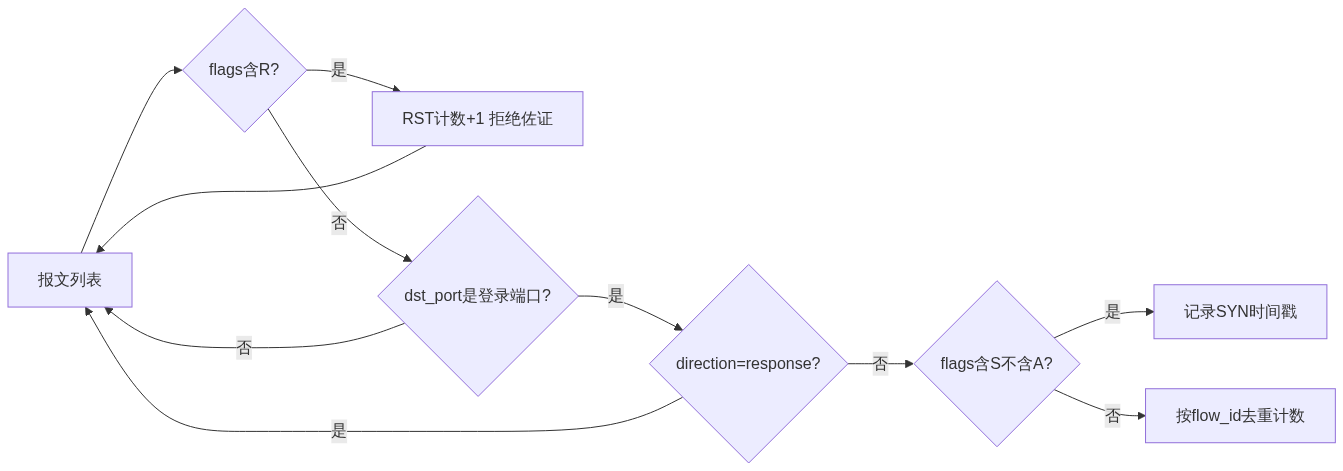
\includegraphics[width=0.85\textwidth]{figures/08_bruteforce_collect.png}
\caption{\_collect\_attempts 连接尝试收集流程}
\label{fig:bf-collect}
\end{figure}

\textbf{双模式计数策略}：
\begin{enumerate}[nosep]
    \item \textbf{优先SYN计数}：flags 含``S''且不含``A''的报文视为一次新建连接尝试。一次 SYN = 一次 TCP 握手发起，直接对应一次登录尝试。
    \item \textbf{退化flow\_id去重}：当 flags 字段缺失时，退化为按不同 flow\_id 计数，同一 flow\_id 的多个数据包只计一次，防止重复计数。
\end{enumerate}

\textbf{RST拒绝佐证}：
\begin{itemize}[nosep]
    \item 监测方向为受害目标 $\to$ 攻击源的 RST 报文（flags 含``R''，src\_port 为登录端口）
    \item 统计值在告警中作为``连接被拒绝次数''出现，证明认证失败
\end{itemize}

\subsection{滑动窗口密度统计（\_max\_count\_in\_window）}

双指针滑动窗口算法求任意 60 秒窗口内的最大连接尝试密度：
\begin{itemize}[nosep]
    \item 时间复杂度 O(n)，空间复杂度 O(1)
    \item 维护 left/right 两个指针，right 向右扩展时 left 收缩确保窗口 $\le$ window\_sec
    \item 返回 (窗口内最大事件数, 该窗口最后事件的时间戳)
\end{itemize}

\begin{figure}[H]
\centering
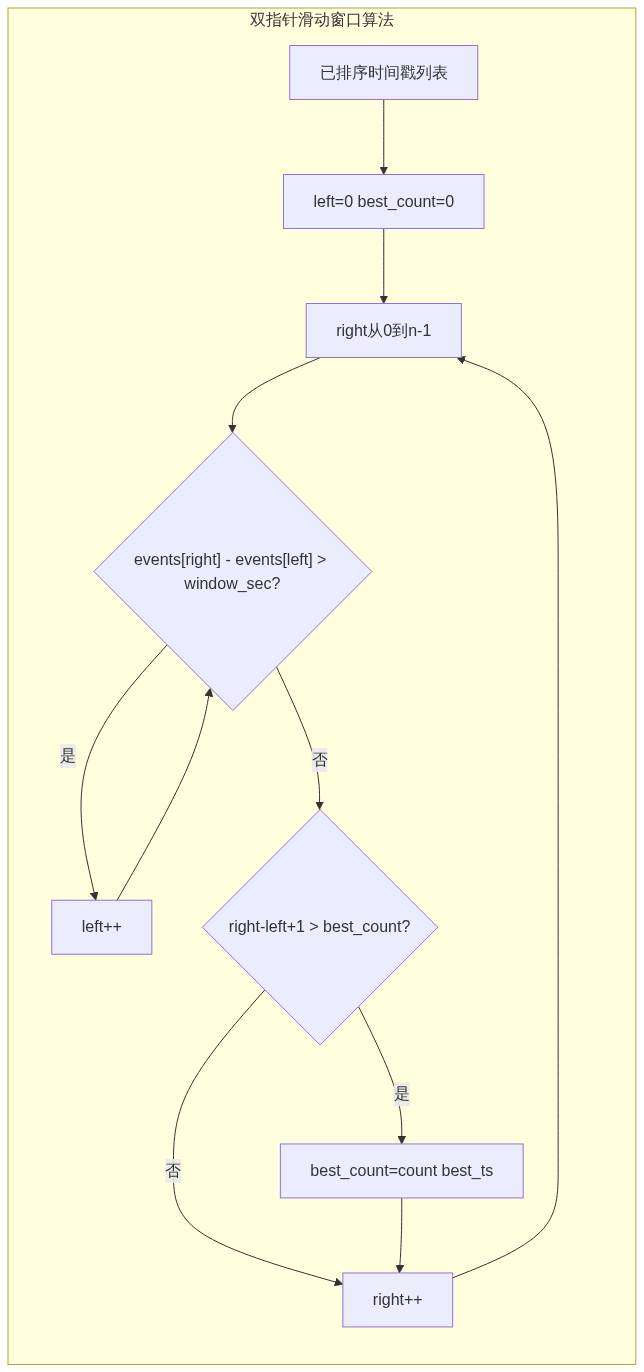
\includegraphics[width=0.7\textwidth]{figures/09_sliding_window.png}
\caption{双指针滑动窗口算法}
\label{fig:sliding}
\end{figure}

\subsection{告警产出}

\begin{itemize}[nosep]
    \item \textbf{严重度分档}：窗口内尝试次数达到 threshold（默认10）$\to$ medium；达到 2$\times$threshold（20）$\to$ high
    \item \textbf{端口 $\to$ 服务名映射}：21$\to$FTP, 22$\to$SSH, 23$\to$Telnet, 3389$\to$RDP, 3306$\to$MySQL, 5432$\to$PostgreSQL, 6379$\to$Redis
    \item \textbf{告警描述（行为导向）}：``检测到针对 SSH 服务(22端口)的暴力破解行为，攻击源 X 在 60 秒内向 Y 发起 18 次连接尝试，超出基线阈值 10 次，其中 18 次连接被目标拒绝(RST)，疑似认证失败''
    \item \texttt{behavior\_id = alert\_id}（每个分组即一个攻击行为事件）
    \item 输出字段集严格对齐 \texttt{docs/interface\_spec.md} 的 Alert Record schema
\end{itemize}

\textbf{CLI入口}：
\begin{lstlisting}
python -m src.bruteforce_detect.login_monitor \
    --input mock_data/mock_packets.json \
    --output results/bruteforce_alerts.json \
    --window 60 --threshold 10
\end{lstlisting}

% ============================================================
% 七、模块四：异常行为检测
% ============================================================
\section{系统功能模块四：异常行为检测模块（姜新晨）}

\subsection{模块结构}

\begin{verbatim}
src/anomaly_detect/
├── __init__.py
├── baseline.py              # 基线配置加载
└── anomaly_detector.py      # 端口扫描 + 异常外联 + CLI
\end{verbatim}

\subsection{基线配置（baseline.py）}

\texttt{load\_config(config\_path)} 从 \texttt{config/baseline\_config.json} 读取阈值配置，文件不存在时返回空字典并使用代码中默认值，不崩溃。

配置文件结构：
\begin{lstlisting}
{
  "port_scan": {
    "time_window_sec": 60,
    "unique_dst_port_threshold": 20
  },
  "external_connection": {
    "internal_networks": ["192.168.0.0/16", "10.0.0.0/8", "172.16.0.0/12"]
  },
  "lateral_movement": {
    "time_window_sec": 300,
    "internal_dst_count_threshold": 10
  }
}
\end{lstlisting}

\subsection{端口扫描检测}

以 \texttt{src\_ip} 为分组维度，统计在 \texttt{time\_window\_sec}（默认60秒）窗口内该 IP 访问过的不同 \texttt{dst\_port} 集合。当 \texttt{len(unique\_dst\_ports) >= unique\_dst\_port\_threshold}（默认20）时产生告警。

\begin{itemize}[nosep]
    \item \texttt{dst\_network} 字段填入被扫描的内网网段 CIDR 表示法
    \item \texttt{category = "端口扫描"}，\texttt{detector = "anomaly"}
    \item \texttt{severity} 按偏离程度分级
\end{itemize}

\begin{figure}[H]
\centering
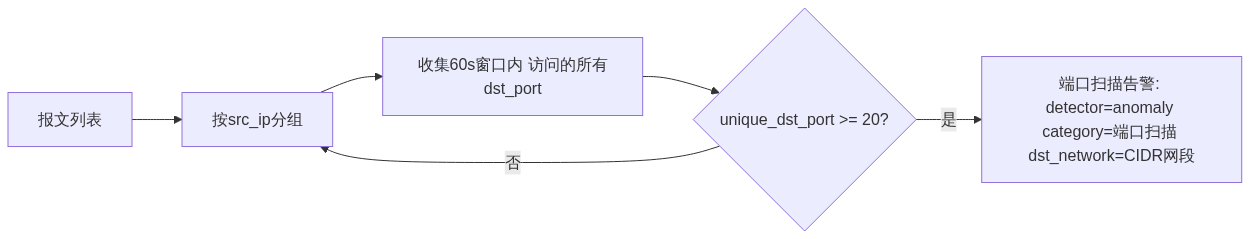
\includegraphics[width=\textwidth]{figures/13_scan_detection.png}
\caption{端口扫描检测流程}
\label{fig:scan}
\end{figure}

\subsection{异常外联检测}

判断条件：
\begin{enumerate}[nosep]
    \item \texttt{src\_ip} 属于内网IP段（10.0.0.0/8, 172.16.0.0/12, 192.168.0.0/16）
    \item \texttt{dst\_ip} 不属于上述任一内网段
\end{enumerate}

满足条件的每个唯一 \texttt{(src\_ip, dst\_ip)} 对产生一条告警，\texttt{severity = "medium"}。

\begin{figure}[H]
\centering
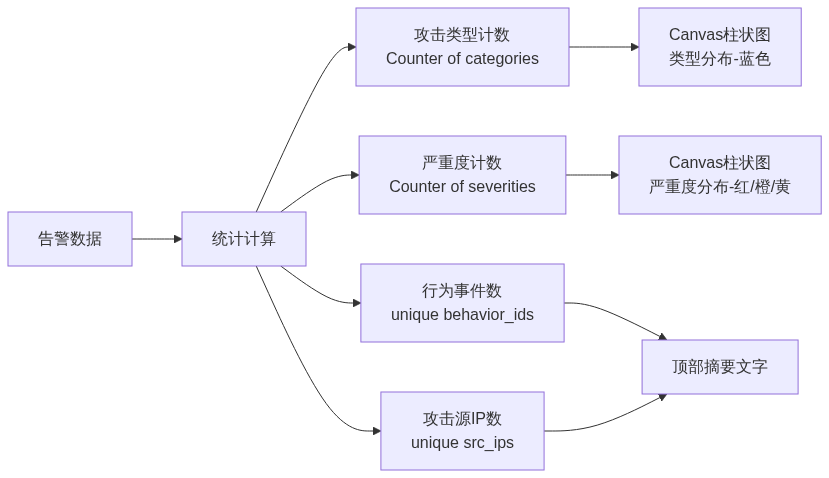
\includegraphics[width=\textwidth]{figures/17_external_connection.png}
\caption{异常外联检测流程}
\label{fig:external}
\end{figure}

\textbf{CLI入口}：
\begin{lstlisting}
python -m src.anomaly_detect.anomaly_detector \
    --input mock_data/mock_packets.json \
    --output results/anomaly_alerts.json
\end{lstlisting}

% ============================================================
% 八、模块五：告警汇总与监控GUI
% ============================================================
\section{系统功能模块五：告警汇总与监控GUI（韩宇飞）}

\subsection{模块结构}

\begin{verbatim}
src/gui_alert/
├── __init__.py
├── aggregator.py       # 汇总 + 去重 + 行为关联
└── gui.py              # tkinter 三页签 GUI
\end{verbatim}

\begin{figure}[H]
\centering
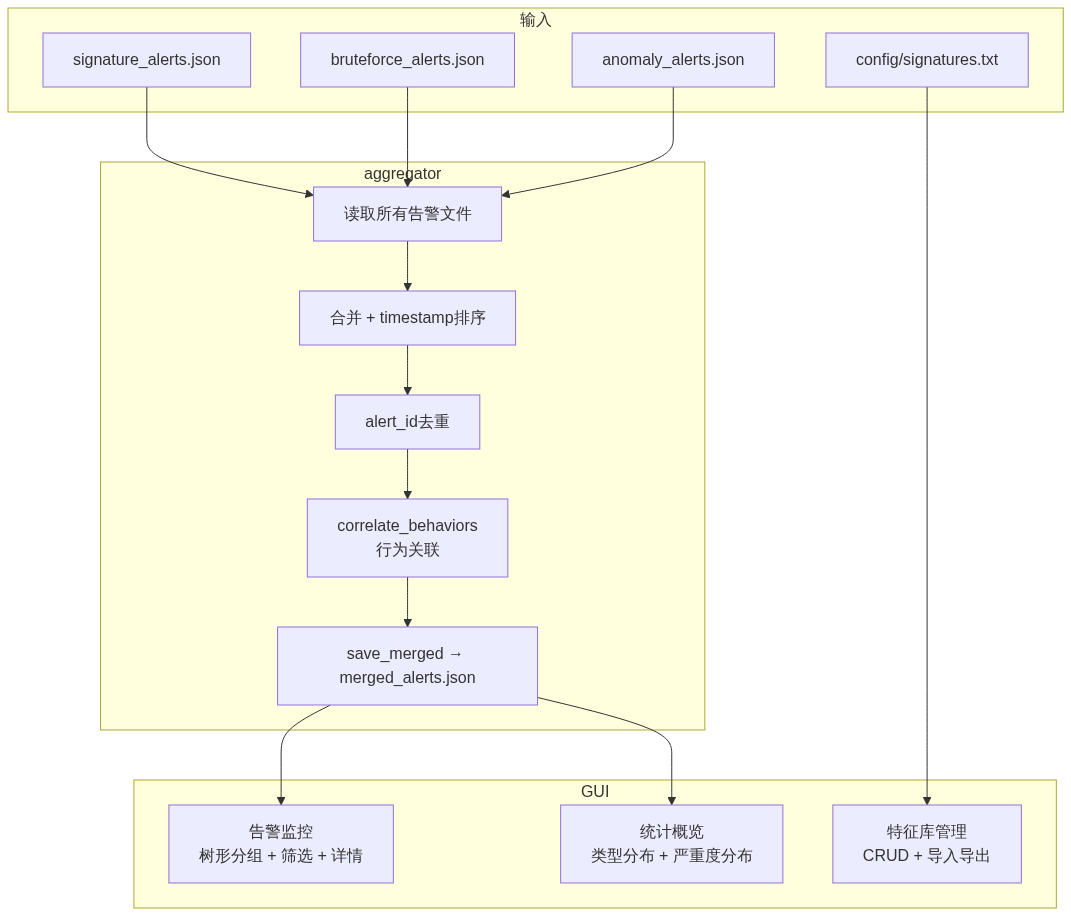
\includegraphics[width=\textwidth]{figures/14_aggregator_module.png}
\caption{aggregator + GUI 模块结构与数据流}
\label{fig:agg-module}
\end{figure}

\subsection{行为关联汇总（aggregator.py）}

\texttt{aggregate(alert\_files)} 处理流程：

\begin{enumerate}[nosep]
    \item \textbf{加载}：遍历 \texttt{alert\_files} 列表，逐个 JSON 反序列化，文件缺失/格式异常时打印 WARNING 跳过，不中断。
    \item \textbf{合并排序}：将所有告警按 \texttt{timestamp} 升序排列。
    \item \textbf{去重}：以 \texttt{alert\_id} 为键去重，重复的 \texttt{alert\_id} 仅保留首次出现者。
    \item \textbf{行为关联}：调用 \texttt{correlate\_behaviors(alerts, time\_window\_sec=60)}。
\end{enumerate}

\begin{figure}[H]
\centering
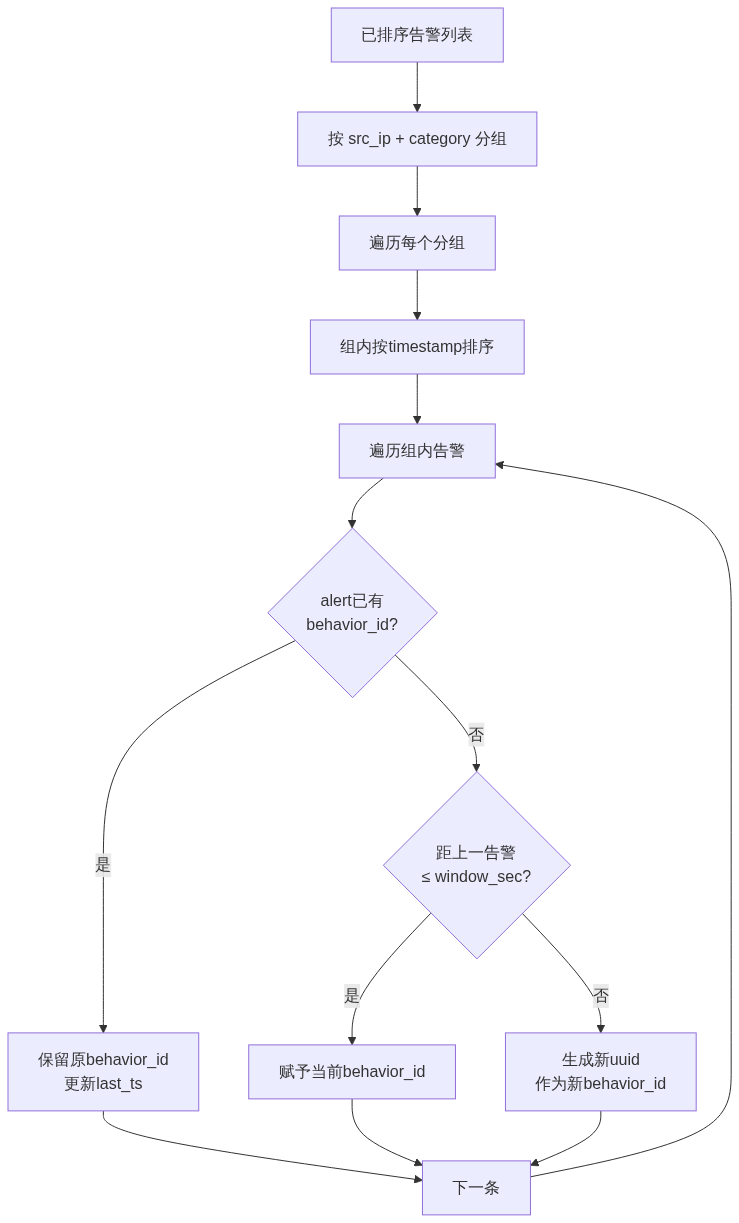
\includegraphics[width=\textwidth]{figures/15_correlate_behaviors.png}
\caption{correlate\_behaviors 行为关联算法}
\label{fig:correlate}
\end{figure}

\textbf{关联规则}：
\begin{itemize}[nosep]
    \item 同一 \texttt{src\_ip} + 同一 \texttt{category} + 时间间隔 $\le$ 60秒 $\to$ 同一 \texttt{behavior\_id}
    \item 检测模块已自行标注 \texttt{behavior\_id} 的告警，aggregator 保留原值不覆盖
    \item 跨 detector 的同源同类告警也会被关联
\end{itemize}

\subsection{图形监控界面（gui.py）}

\begin{figure}[H]
\centering
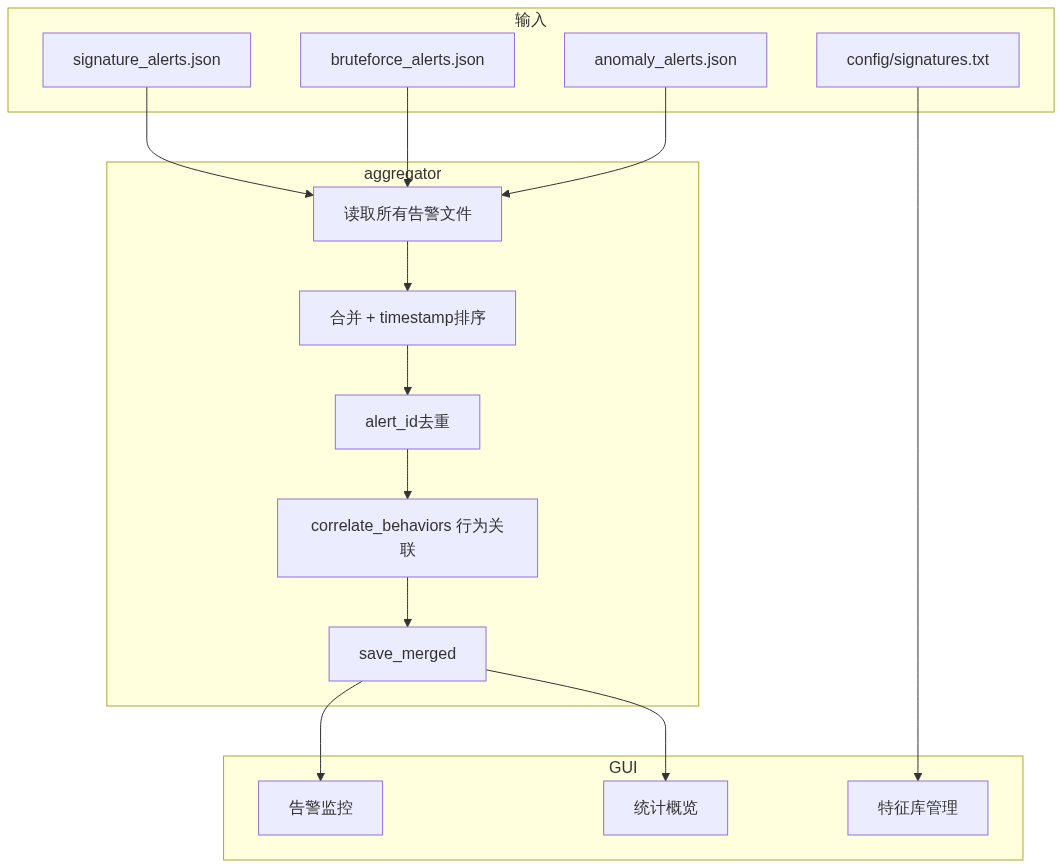
\includegraphics[width=\textwidth]{figures/18_gui_structure.png}
\caption{GUI 三页签结构}
\label{fig:gui}
\end{figure}

基于 tkinter + ttk 实现，零外部依赖，三个页签：

\textbf{页签一「告警监控」}：
\begin{itemize}[nosep]
    \item 按 \texttt{behavior\_id} 分组树形展示告警列表，行为头行灰色粗体标识
    \item 筛选栏：检测器下拉（全部/signature/bruteforce/anomaly）、严重度多选（high/medium/low）、全文搜索输入框
    \item 点击任意告警行在右侧 JSON 详情面板显示完整告警记录
    \item 单条告警行按 severity 着色（high红/orange橙/low黄）
    \item 底部状态栏显示已加载告警总数 + 攻击行为事件数
    \item 30秒定时自动刷新
\end{itemize}

\textbf{页签二「特征库管理」}：
\begin{itemize}[nosep]
    \item 表格展示 \texttt{config/signatures.txt} 中所有规则
    \item 工具栏：[+新增] [编辑] [删除] [导入] [导出] [保存到文件]
    \item 新增/编辑：弹出 Toplevel 表单（6字段输入，combobox 下拉选择匹配模式和严重度）
    \item 导入：文件选择对话框，读取外部 .txt 文件
    \item 导出/保存：按6字段格式写回文件（\texttt{|} 分隔）
\end{itemize}

\textbf{页签三「统计概览」}：
\begin{itemize}[nosep]
    \item Canvas 自绘柱状图（攻击类型分布 + 严重度分布），无需 matplotlib 等额外依赖
    \item 顶部摘要文字：告警总数、攻击行为事件数、涉及攻击源 IP 数
    \item 颜色统一：high=\#dc3545红、medium=\#fd7e14橙、low=\#ffc107黄、图表柱=\#4e73df蓝
\end{itemize}

\textbf{启动方式}：
\begin{lstlisting}
# 全链路运行（检测+汇总+GUI）
python main.py --input mock_data/mock_packets.json
# 仅启动GUI（读取已有告警文件）
python main.py --gui-only
\end{lstlisting}

% ============================================================
% 九、接口设计
% ============================================================
\section{接口设计}

所有模块通过两个标准化 JSON Schema 通信。详细规范见 \texttt{docs/interface\_spec.md}。

\subsection{报文记录格式（Packet Record）}

由 capture 模块产出，三个检测模块统一消费。

\begin{lstlisting}
{
  "timestamp": "2026-07-08T10:00:00.123",
  "flow_id": "192.168.1.10:51234->192.168.1.20:80/TCP",
  "src_ip": "192.168.1.10",
  "src_port": 51234,
  "dst_ip": "192.168.1.20",
  "dst_port": 80,
  "protocol": "TCP",
  "direction": "request",
  "flags": "PA",
  "payload": "GET /login.php?id=1 UNION SELECT ...",
  "payload_len": 128
}
\end{lstlisting}

\begin{table}[H]
\centering
\caption{Packet Record 字段定义}
\small
\begin{tabular}{@{}lp{2.5cm}p{7cm}@{}}
\toprule
字段 & 类型 & 说明 \\
\midrule
\texttt{timestamp}  & string(ISO8601) & 报文捕获时间，精确到毫秒 \\
\texttt{flow\_id}    & string & 五元组流标识，格式 src\_ip:src\_port->dst\_ip:dst\_port/protocol \\
\texttt{src\_ip}     & string & 源IP地址 \\
\texttt{src\_port}   & int    & 源端口，ICMP/ARP无端口协议为null \\
\texttt{dst\_ip}     & string & 目的IP地址 \\
\texttt{dst\_port}   & int    & 目的端口 \\
\texttt{protocol}    & string & TCP / UDP / ICMP / ARP \\
\texttt{direction}   & string & request / response \\
\texttt{flags}       & string & TCP标志位：S/A/P/F/R 组合 \\
\texttt{payload}     & string & 应用层载荷，二进制用 \textbackslash xNN 转义 \\
\texttt{payload\_len}& int    & 线路上原始payload字节长度 \\
\bottomrule
\end{tabular}
\end{table}

\subsection{统一告警格式（Alert Record）}

由三个检测模块产出，aggregator 消费。

\begin{lstlisting}
{
  "alert_id": "b3f1a2c4-1234-4abc-9def-000000000001",
  "behavior_id": "b3f1a2c4-1234-4abc-9def-000000000001",
  "detector": "signature",
  "category": "Web攻击/SQL注入",
  "src_ip": "192.168.1.10",
  "src_port": 51234,
  "dst_ip": "192.168.1.20",
  "dst_network": null,
  "dst_port": 80,
  "severity": "high",
  "description": "检测到针对 /login.php 的 SQL 注入攻击行为...",
  "evidence": "GET /login.php?id=1 UNION SELECT ...",
  "timestamp": "2026-07-08T10:00:01.000"
}
\end{lstlisting}

\begin{table}[H]
\centering
\caption{Alert Record 字段定义}
\small
\begin{tabular}{@{}lp{2.5cm}p{7.5cm}@{}}
\toprule
字段 & 类型 & 说明 \\
\midrule
\texttt{alert\_id}    & string(uuid) & 全局唯一告警ID \\
\texttt{behavior\_id}  & string(uuid) & 攻击行为事件标识（同源同类关联） \\
\texttt{detector}      & string & signature / bruteforce / anomaly \\
\texttt{category}      & string & 攻击类型简述 \\
\texttt{src\_ip}       & string & 攻击源IP \\
\texttt{src\_port}     & int    & 攻击源端口 \\
\texttt{dst\_ip}       & string & 受害目标IP \\
\texttt{dst\_network}   & string & CIDR网段（端口扫描/横向扩散时填写） \\
\texttt{dst\_port}     & int    & 受害目标端口 \\
\texttt{severity}      & string & low / medium / high \\
\texttt{description}   & string & \textbf{攻击行为描述}（行为导向语态，非特征罗列） \\
\texttt{evidence}      & string & 匹配原始内容或统计证据 \\
\texttt{timestamp}     & string(ISO8601) & 告警产生时间 \\
\bottomrule
\end{tabular}
\end{table}

\subsection{统一函数签名}

所有检测模块必须遵循同一函数签名：

\begin{lstlisting}
def detect(packets: list[dict]) -> list[dict]:
    """
    Args:
        packets: 符合 Packet Record 格式的列表
    Returns:
        符合 Alert Record 格式的列表（无告警时返回 []，不返回 None）
    """
\end{lstlisting}

\subsection{统一日志规范}

所有模块使用 Python 标准库 \texttt{logging}：

\begin{lstlisting}
import logging
logger = logging.getLogger(__name__)

logging.basicConfig(
    level=logging.INFO,
    format="[%(name)s] %(levelname)s %(asctime)s %(message)s",
)
\end{lstlisting}

\begin{itemize}[nosep]
    \item \texttt{logger.debug()} — 调试信息（如跳过单条报文的原因）
    \item \texttt{logger.info()} — 正常流程信息（如``已加载 N 条规则''）
    \item \texttt{logger.warning()} — 非致命异常（文件缺失、字段缺失）
    \item \texttt{logger.error()} — 致命错误（scapy 未安装）
    \item 禁止使用 \texttt{print()} 调试（CLI 结束时的摘要除外）
\end{itemize}

% ============================================================
% 十、开发平台
% ============================================================
\section{开发平台}

\subsection{软件平台}

\begin{table}[H]
\centering
\caption{软件平台选型}
\begin{tabular}{@{}lll@{}}
\toprule
项目 & 选型 & 版本要求 \\
\midrule
开发语言   & Python                 & $\ge$ 3.9 \\
抓包库     & scapy                  & $\ge$ 2.5.0 \\
GUI框架    & tkinter                & Python 标准库 \\
测试框架   & pytest                 & $\ge$ 7.0 \\
版本控制   & Git + GitHub Flow      & — \\
代码格式化 & black + isort          & $\ge$ 24.0 / $\ge$ 5.13（推荐） \\
\bottomrule
\end{tabular}
\end{table}

注意：不使用 Python 3.10+ 独有语法（如 match/case），保持向下兼容 Python 3.9。

\subsection{硬件平台}

\begin{itemize}[nosep]
    \item 最低配置：双核CPU、4GB内存、10GB可用磁盘空间
    \item 推荐配置：四核CPU、8GB内存、SSD硬盘
    \item 网络：实时抓包需网卡支持混杂模式
    \item 虚拟化：VirtualBox / VMware / WSL2 均可；虚拟机网络建议桥接模式
    \item 操作系统：Linux（推荐 Ubuntu 22.04 LTS）或 Windows 10/11 + WSL2
\end{itemize}

% ============================================================
% 十一、系统出错处理
% ============================================================
\section{系统出错处理}

\begin{table}[H]
\centering
\caption{异常场景与处理策略}
\begin{tabular}{@{}p{4.6cm}p{5.4cm}p{4.2cm}@{}}
\toprule
异常场景 & 处理策略 & 影响范围 \\
\midrule
输入文件不存在/为空 & 打印 WARNING 日志，返回空列表 \texttt{[]}，不崩溃 & 单模块 \\
报文记录缺失非必填字段 & 按 null 处理，跳过依赖该字段的判断逻辑 & 单条报文 \\
payload 含无法解码的二进制 & \texttt{\textbackslash xNN} 转义保留，不影响其余字段 & 无 \\
数据量不足无法形成统计窗口 & 不产生告警，不报错 & 无 \\
flow\_id 缺失 & 消费模块自行根据五元组构建 & 单模块内部 \\
scapy 未安装 & 打印 ERROR 日志，返回空列表 & capture模块 \\
时间戳无法解析 & 跳过该报文，其余报文正常处理 & 单条报文 \\
JSON 文件格式异常 & 打印 WARNING/ERROR，跳过该文件 & 单文件 \\
GUI 无告警数据 & 状态栏提示``未找到告警文件''，不弹错误对话框 & GUI \\
特征库规则行字段数 $\ne$ 6 & 跳过该行，打印 WARNING & 单条规则 \\
实时抓包权限不足 & 打印 ERROR，提示需 root/管理员权限 & capture模块 \\
检测模块未产生告警 & 输出空 JSON 数组 \texttt{[]}，aggregator 平滑处理 & 无 \\
\bottomrule
\end{tabular}
\end{table}

\begin{figure}[H]
\centering
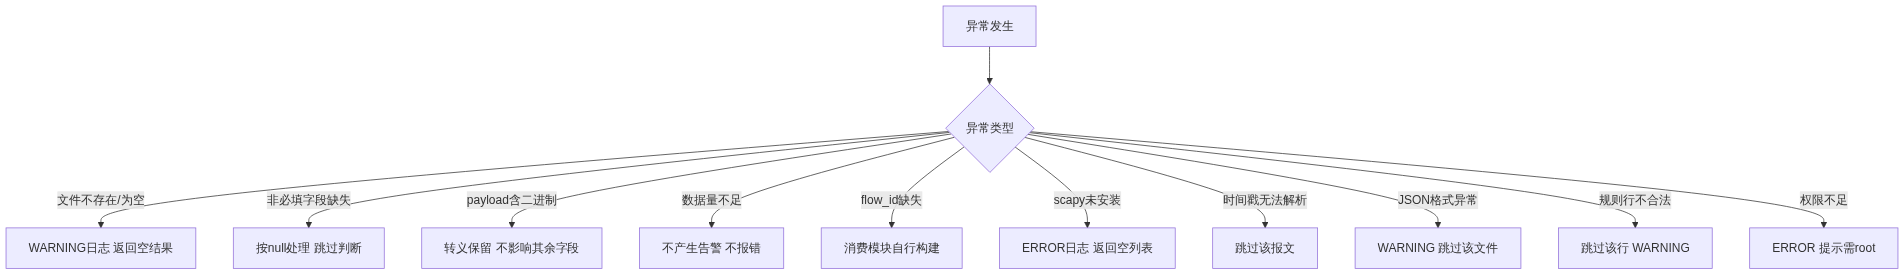
\includegraphics[width=\textwidth]{figures/16_error_handling.png}
\caption{系统出错处理决策树}
\label{fig:error}
\end{figure}

\end{document}
